\chapter{Background \& Related Work}

In this chapter, I first provide a brief introduction to harmony and chords and their role in music. I then discuss the different ways in which music can be represented as input to a machine learning model. This is followed by an overview of the field of automatic chord recognition (ACR). This includes the datasets and models that are commonly used in ACR, the challenges that are faced in this field and future directions.

\section{Background}

\subsection{Harmony and Chords}

Harmony is the combination of simultaneously sounded notes. A common interpretation of such sounds is as a chord. Chords can be thought of as a collection of at least two notes built from a root note and scale. Any notes from the scale can be present but the most common are the third, fifth and seventh. A chord's \emph{quality} is determined by the intervals between notes in the chord irrespective of the root note. The most common qualities are major and minor. Many other qualities exist such as diminished and suspended. Chords can be played in \emph{inversion}, where the root note is not the lowest Note. In this work, chords are represented using Harte notation~\citep{HarteNotation}.

Chords can be closely related. \texttt{C:maj7} is very close to \texttt{C:maj}. The only difference is an added major seventh. An important relation in music theory is between \emph{relative major/minor} chords. These pairs of chords are built from the same scale so share many notes. For example, \texttt{G:maj} and \texttt{E:min} are related in this way. It is possible for chords to share the same set of notes like \texttt{G:maj6} and \texttt{E:min7}.

Chords are an important part of music. They provide harmonic context for a melody and can be used to convey emotion, tension and release~\citep{HarmonyandVoiceLeading}. They are also important for improvisation where musicians will play notes that fit the chord progression~\citep{JazzTheoryBook}. Contemporary guitar music is often represented by a chord sequence. Chords are also important for songwriting and production where a chord progression can form the basis of a song. Music analysis also makes heavy use of chords. The harmonic structure of a piece can be analysed to understand the composer's intentions and why we enjoy the music~\citep{TonalAnalysisBach}.

\subsection{Chord Recognition}

Chord recognition is the task of identifying which chord is playing at any moment in a piece of music. This can be useful for creating notated versions of songs for musicians, musicologists and music recommendation. Those wishing to learn a song may visit websites such as Ultimate Guitar\footnote{\url{https://www.ultimate-guitar.com/}} where users submit chord annotations for songs. Musicologists may wish to analyse the harmonic structure of a piece of music. Music recommendation systems can recommend songs based on their harmonic content as similar music will often have similar harmonic content~\citep{MusicGenreClassification}. For example, modern pop music famously uses many similar chords~\footnote{\url{https://www.youtube.com/watch?v=oOlDewpCfZQ} accessed 25th February 2025} while contemporary jazz music is known for its complex and rich exploration of harmony.

All of the above motivate the need for accurate chord annotations. However, annotations from online sources can be of varying quality and may not be available for all songs~\citep{Choco}. The task of annotating chords is time-consuming and requires a trained musician~\citep{McgillBillboard}. Automatic chord recognition systems have the potential to alleviate these problems by providing a fast, accurate and scalable solution.

Unfortunately, chord recognition is a non-trivial task. Which chord is playing when is inherently ambiguous. Different chords can share the same notes and the same chord can be played in many ways on different instruments. Precisely when a chord starts and ends can be imprecise. Whether a melody note is part of a chord and whether a melody alone is enough to imply harmonic content are both ambiguous. In order to identify a chord, data across time must be considered. For example, a chord may be vamped or arpeggiated. Audio also contains many unhelpful elements for chord recognition such as reverb, distortion and unpitched percussion.

% \begin{figure}[H]
%     \centering
%     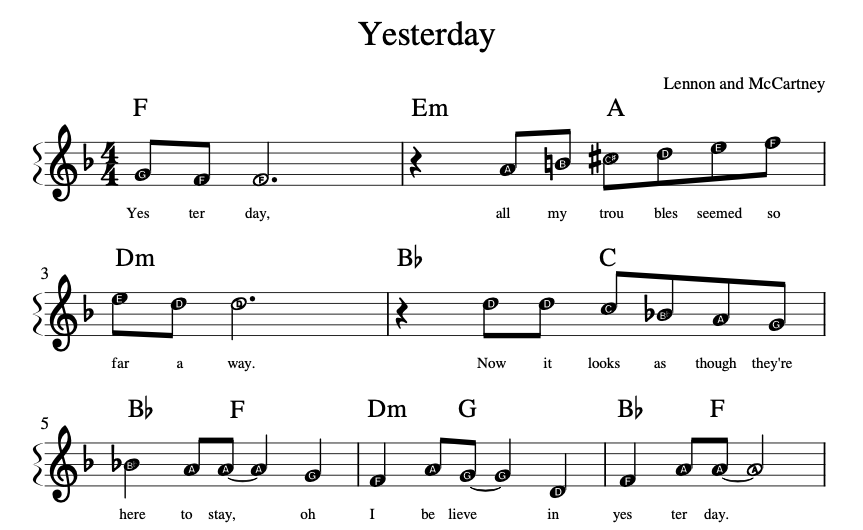
\includegraphics[width=0.6\textwidth]{figures/lead_sheet_example.png}
%     \caption{An example of a lead sheet for `Yesterday' by the Beatles. We can see chords written above the stave and the melody written in standard musical notation. Such a chordal representation is useful for musicians who want to learn and perform songs quickly or improvise around them.}\label{fig:lead_sheet_example}
% \end{figure}

% Lead sheets are most notably used in jazz music where their origins lie. They date back to the mid 20th century, and were originally called `fake sheets' because they were used by musicians to `fake' their way through a song~\citep{RealBookPodcast}. Any jazz musician worth their salt owns a `real book', so called to distinguish it from the fake books that were used in the past. Real books contain lead sheets for hundreds of jazz standards, and are still an essential tool for any seasoned jazz musician. 

% More recently they have served as a useful tool for musicians in other genres too, such as pop and rock, who want to learn and perform songs quickly and easily. They allow efficient communication of the important elements of a song, without the need for a full score, encouraging further improvisation and personalisation of the song.

% Lead sheets do not contain all the information of a full score, such as dynamics, articulation, or specific voicings of chords. Furthermore, they are not suitable for all types of music, such as classical music, where a full score is necessary to convey the composer's intentions, or rap music where the lyrics and beat are normally the most important elements. However, they are a useful tool for many musicians, and are a common way of representing music for both learning and performing.

% \subsection{Automatic Music Transcription}

% Automatic Music Transcription (AMT) is a field within Music Information Retrieval (MIR) that aims to construct models that convert musical audio into symbolic representations.~\citep{ComprehensiveReviewMusicTranscription} provide a comprehensive review of different forms of transcription. For lead sheet transcription, we are interested in their highest level of transcription: notation-level. We want to be able to take an audio recording of a song and generate a lead sheet that contains the melody and harmony of the song. This is a challenging task, as it requires the model to isolate and transcribe a melody, transcribe the chordal information, and then combine these two elements into a coherent lead sheet where the melody and harmony are aligned in time/beat.

% There are three sub-fields of musical transcription that are of interest to lead sheet generation: Automatic Chord Recognition (ACR), Melody Transcription (previously called F0 estimation) and Beat Detection.


\subsection{Music Features}\label{sec:background-features}

Recorded music can be represented in a variety of ways on a computer. The simplest is as a raw time-series of amplitudes, referred to as the audio's waveform. Data in the raw audio domain has been applied in generative models such as Jukebox~\citep{Jukebox} and MusicGen~\citep{MusicGen} and autoencoders~\citep{Encodec}.

\textbf{Spectrogram}: A spectrogram is a transformation of a waveform into the time-frequency domain calculated via a short-time Fourier transform (SFTF). Spectrograms are commonly used in many audio processing tasks such as audio search~\citep{ShazamSpectrogram} and music transcription~\citep{PianoTranscriptionWithTransformer}. As of yet, linear spectrograms computed using the STFT have not been used in ACR tasks~\citep{20YearsofACR}.

\textbf{CQT}: A common version of the spectrogram used in music transcription is the constant-Q transform (CQT)~\citep{CQT}. The CQT is another version of the spectrogram with frequency bins that are logarithmically spaced and bin widths that are proportional to the frequency. This is motivated by the logarithmic nature of how humans perceive pitch intervals in music: a sine wave with double the frequency is perceived as one octave higher. As such, CQTs are used in many music transcription tasks and are very popular for ACR~\citep{FirstDeepLearningCQT,StructuredTraining}. An example CQT from the dataset used in this work is shown in Figure~\ref{fig:cqt_example}. As \citet{SaliencyChroma} note, CQTs are preferred to other spectrograms for ACR due to their finer resolution at lower frequencies and for their ease with which pitches can be studied and manipulated. For example, CQTs make pitch shifting possible through a simple shift of the CQT bins. Another logarithmic variant of the spectrogram is the mel-spectrogram, based on the mel-scale~\citep{MelScale}. It is intended to mimic the human ear's perception of sound and is commonly used in speech recognition~\citep{SpeechProcessingMels} but has also been used in music transcription tasks~\citep{MelodyTranscriptionViaGenerativePreTraining}.

% \textbf{Mel-spectrogram}: A common alternative to the standard linear spectrogram is the mel-spectrogram. The only difference is that the frequency scale is no longer linear. This transformation uses the mel-scale~\citep{MelScale}. The scale was constructed using estimates of human perception of different frequencies. It is approximately linear below 1kHz and logarithmic above. The mel-spectrogram is commonly used in speech recognition~\citep{SpeechProcessingMels} and has also been used in music transcription tasks~\citep{MelodyTranscriptionViaGenerativePreTraining}.


\begin{figure}[h]
    \centering
    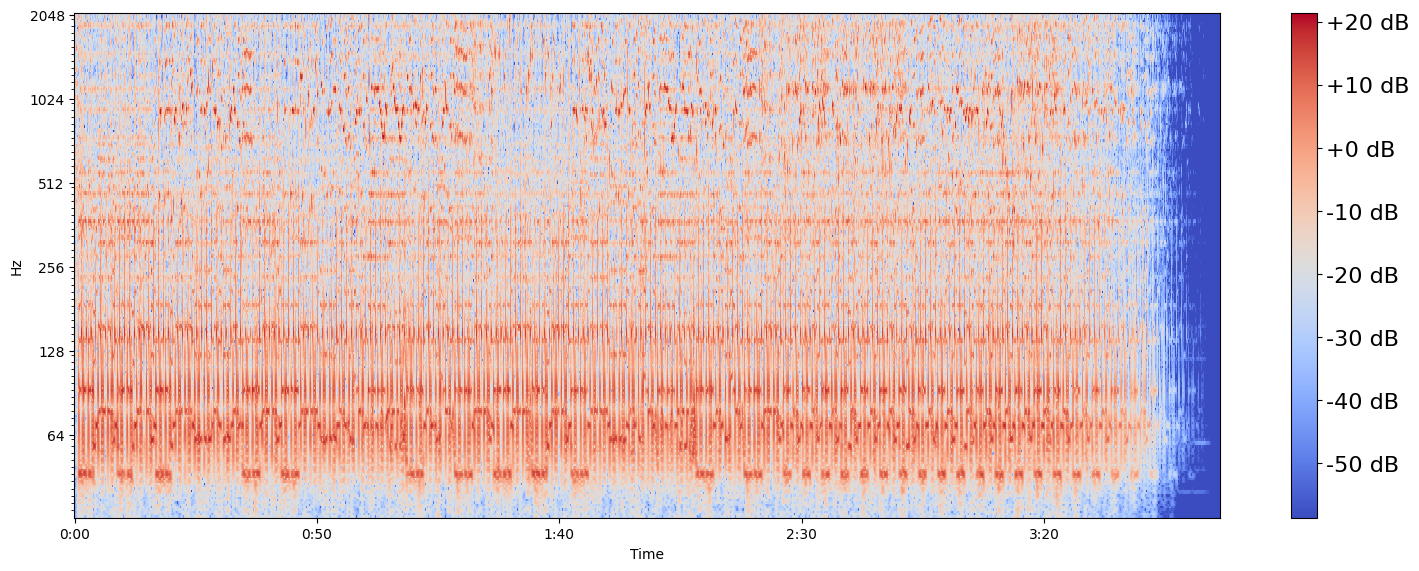
\includegraphics[width=0.8\textwidth]{figures/sample_cqt.png}
    \caption{CQT of `Girls Just Wanna Have Fun' by Cyndi Lauper. We can see the log-spaced frequency bins on the y-axis. There is clear structure and repetition in the song, particularly in the lower frequencies, which can be attributed to a regular drum groove. Such structure gives an idea of the patterns a machine learning model may look for to identify chords.}~\label{fig:cqt_example}
\end{figure}

\textbf{Chroma Vectors}: Chroma vectors are a 12-dimensional time-series representation, where each dimension corresponds to a pitch class. Each element represents the strength of each pitch class in the Western chromatic scale. Such features have been generated by deep learning methods~\citep{BalanceRandomForestACR} or by hand-crafted methods~\citep{NNLSChroma,librosa} and have seen use in recent ACR models~\citep{HarmonyTransformer}. A representation of a song as a chroma vector over time can be thought of as a another type of spectrogram, referred to as a \emph{chromagram}.

\textbf{Generative Features}: More recently, features extracted from generative music models have been used as input. I refer to such features as \emph{generative features}. The proposed benefit is that the vast quantities of data used to train these models requires rich representations of the music. These features have been shown to contain useful information for music information retrieval (MIR) tasks~\citep{GenerativeFeaturesforMIR}. \citet{MelodyTranscriptionViaGenerativePreTraining} use features from JukeBox~\citep{Jukebox} to train a transformer~\citep{AttentionIsAllYouNeed} for both melody transcription and chord recognition. They found that these features outperformed mel-spectrograms in melody transcription tasks but did not report results for ACR nor with CQTs.


% Related Work
\section{Related Work}\label{sec:related_work}

The field of ACR has seen considerable research since the seminal work of \citet{FujishimaACR} in 1999. Below, I provide a brief overview of the field over the last 15 years including the datasets, metrics and models and representations of time that are commonly used. I conclude by discussing some of the common challenges faced and motivating the research carried out in this project. 

\subsection{Data}\label{sec:background-data}

Sources of data that have seen common use in ACR relevant to this work include:

\begin{itemize}
    \item \emph{Mcgill Billboard}: over 1000 chord annotations of songs randomly selected from the Billboard `Hot 100' Chart between 1958 and 1991.~\citep{McgillBillboard}
    \item \emph{Isophonics}: 300 annotations of songs from albums by The Beatles, Carole King and Zweieck.~\citep{Isophonics}
    \item \emph{RWC-Pop}: 100 pop songs with annotations available\footnote{\url{https://github.com/tmc323/Chord-Annotations}} for chords.~\citep{RWC}
    \item \emph{USPop}: 195 annotations of songs chosen for popularity.~\citep{USPop}
    \item \emph{JAAH}: 113 annotations of a collection of jazz recordings.~\citep{JAAH}
    \item \emph{HookTheory}: 50 hours of labelled audio in the form of short musical segments, crowdsourced from an online forum called HookTheory\footnote{https://www.hooktheory.com/}.~\citep{MelodyTranscriptionViaGenerativePreTraining}
\end{itemize}

Many of these have been compiled together into the \emph{Chord Corpus} by \citet{Choco} with standardised annotation formats. However, audio is scarce, in part due to copyright issues. The most common dataset is comprised of 1217 songs compiled from the first four of the above collections. This dataset is dominated by pop songs.

Another problem is that the existing data is imbalanced, with a large number of major and minor chords and fewer instances of chords with more obscure qualities. This can lead to models that are biased towards predicting major and minor chords. Attempts to address such an imbalanced distribution have been made by weighting the loss function~\citep{ACRLargeVocab1}, adding `structure' to the chord targets~\citep{StructuredTraining,ACRLargeVocab1}, re-sampling training examples to balance chord classes~\citep{BalanceRandomForestACR} and curriculum learning~\citep{CurriculumLearning}.

\textbf{Pitch Augmentation}: Due to the lack of labelled data, data augmentation via pitch shifting has been applied to ACR. Input features are pitch shifted while chords are transposed. \citet{StructuredTraining} note the large increase in performance using pitch shifting directly on the audio. Other works have since used pitch shifting directly on the CQT~\citep{ACRLargeVocab1}. No work has compared the two methods.

\textbf{Synthetic Data Generation}: Data has been scaled up using augmentation and semi-supervised learning with some success~\citep{ScalingUpSemiSupervisedLearning}. Research has been done into the use of synthetic data~\citep{MusicGenTrainingData,AnnotationFreeSyntheticData} and self-supervised learning~\citep{MERTSupervisedLearning} for other MIR tasks but not for ACR. With the advent of new models which accept chord-conditioned input~\citep{MusiConGen}, the possibility of generating synthetic data for ACR is an exciting avenue of research.

% \subsection{Evaluation}

% Evaluation is typically done using weighted chord symbol recall (WCSR). This is defined as the recall of each chord class weighted by its duration. Simply put, this is the fraction of time that the prediction is correct. We define this more formally in Section~\ref{sec:evaluation}. More music-aware measures of recall provide further insights such as the recall of the correct root note, third, seventh or mirex, a metric which checks whether a predicted chord has at least 3 notes in common with the true chord. These metrics are implemented by \citet{mir_eval} in the \texttt{mir\_eval} library.\footnote{\url{https://mir-evaluation.github.io/mir_eval/}} 

% Other metrics targeting the imbalanced nature of the data have been proposed. These include the mean accuracy over classes and qualities. However, these metrics are defined in terms of discrete frames. I propose a definition in continuous time, similar to WCSR.

% Some works also do a little qualitative evaluation. \citet{MelodyTranscriptionViaGenerativePreTraining} provide examples of the lead sheets their model produces and categorises failure modes. However, most works focus solely on improving quantitative metrics and conducting analysis on the internal elements of the model. There is a lack of focus on the kinds of errors their models makes and on the utility of the model in real-world applications.

\subsection{Models}

\textbf{Model Architectures}: Since the work of \citet{RethinkingChordRecognition}, chord recognition has been predominantly tackled by deep learning architectures. The authors used a convolutional neural network (CNN) to classify chords from a CQT. CNNs have been combined with recurrent neural networks (RNNs)~\citep{ACRCNNRNN1,ACRLargeVocab1,StructuredTraining} with a CNN performing feature extraction from a spectrogram and an RNN sharing information across frames. More recently, transformers have been applied in place of the RNN~\citep{MelodyTranscriptionViaGenerativePreTraining, HarmonyTransformer, AttendToChords,ChordFormer,CurriculumLearning,BTC}.

Despite increasingly complex models being proposed, performance has not improved significantly. In fact, \citet{BTC} found that their transformer performed marginally worse than a CNN. \citet{FourTimelyInsights} talk of a 'glass ceiling' with increases in performance stagnating after the advent of deep learning in ACR. This was 10 years ago and the situation has not changed significantly. Despite this, continued efforts have been made to develop complex models with the sole motivation of improving performance, with mixed success. This has lead to overly complex ACR models seeing use in this other MIR tasks such as chord-conditioned generation where \citet{MusiConGen} use the model developed by \citet{BTC} despite its lack of improvement over simpler predecessors. Furthermore, there is little comparison to simple baselines to provide context for the performance gain associated with increasing model complexity.

\textbf{Decoding}: A decoding step is often performed on the probabilities outputted by the neural network. This can smooth predictions and share information across frames. Decoding follows the Viterbi algorithm to find the most likely sequence of chords given the model's output. \citet{BalanceRandomForestACR} use a hidden Markov model (HMM), treating the probability distributions over chords generated by the model as emission probabilities and constructing a hand-crafted transition function.  Other works have used conditional random fields (CRF) instead to model the dependencies between chords~\citep{ACRLargeVocab1}. Both methods have used learned statistics and simpler homogeneous penalties between different chords for transitions to different chords. It is unclear which method is better. In both cases, self-transition probabilities are very large and \citet{CommonVariations} argue that increases in performance can be mostly attributed to the reduction in the number of transition. However, more recent analysis of such behaviour is missing from the literature.

\textbf{Model Analysis}: \citet{FeatureMaps} visualise the outputs of layers of the CNN and find that some feature maps correspond to the presence of specific pitches and intervals. \citet{SaliencyChroma} visualise the importance of different parts of an input CQT using saliency maps, noting the clear correlation between pitch classes present in a chord and the saliency maps. Confusion matrices over chord roots and qualities are also commonly used to analyse the performance of models. For example, \citet{StructuredTraining} found that similar qualities are often confused with each other and that the model favours the most common chord qualities. ~\citet{BTC} attempt to interpret attention maps produced by their transformer as musically meaningful.

Regardless of such analyses, too much effort is spent on motivating complex model architectures with a focus on minor improvements in performance. In this work, I will conduct a thorough analysis of an existing model. I will take inspiration from some of the analyses above, while adding a more nuanced understanding of the model's behaviour and failure modes by way of example.

\subsection{Frames and Beats}

Chords exist in time. How the time dimension is processed prior to being fed into the model matters. When audio is  transformed into a spectrogram, each vector of frequencies represents a fixed length of time, called a \emph{frame}. The frame length is determined by hop length used when calculating the CQT. Constant frame lengths can be made short enough such that the constraint imposed on the model to output chord predictions on a per-frame basis is not limiting. However, different hop lengths have been used, varying from 512~\cite{ACRLargeVocab1} up to 4096~\citep{StructuredTraining}. Which hop length works best remain unclear.

More recently, \citet{MelodyTranscriptionViaGenerativePreTraining} used a frame length determined by beats detected from the audio. Because they focus primarily on melody transcription, they define frames to be a 1/16th note $\approx 125$ms with 120 beats per minute (BPM). Such beat synchronicity has been proposed for chord recognition. The underlying assumption is that chords tend to change on the beat. This reduces the computational cost of running the model due to a decreased frame rate and more importantly provides a far more musically meaningful interpretation to the output. However, \citet{CommonVariations} and \citet{RelativePerformance} argue that because beat detection is far from perfect, restricting frames to beats can hurt performance. Beat detection models have improved since then. Proper analysis of beat-synchronous chord recognition in the modern setting is lacking from the literature.  \citet{ChorusAlignmentJAAH} jointly estimate beats and chords but use a different jazz-specific dataset and do not conduct analysis on how beat-wise predictions affect performance.

\subsection{Future Directions}

\citet{20YearsofACR} provide an overview of ACR up to 2019 since the seminal work of \citet{FujishimaACR} in 1999 and provide suggestions for future avenues of research. They look at future research directions. This includes the use of different representations for both audio and chords, of addressing the mismatch between chord changes and discretised frames fed to a model, looking at the larger structures in music like verses and chords, incorporating other elements of the music such as melody and genre, methods of handling subjectivity of chords and the imbalance present in chord datasets. Since then, different works have addressed some of these problems in various ways. Among these problems, the focus has been primarily on addressing the imbalance in the chord dataset. 

In this work, I will implement a simple model that remains competitive with the state-of-the-art~\citep{StructuredTraining}. I will then conduct a thorough analysis of the model and its architecture. I will look at common methods for improving ACR models with more detailed analyses than have previously been conducted. This  analysis will provide insight into the strengths and weaknesses of such models. It may also provide guidance for further improvements. I will also look at novel methods of improvement made possible through generative and beat detection models. This includes the use of generative features and synthetic data as input to the model as well as the use of beat-synchronous frames. Finally, I will evaluate the improved models in terms of their performance in-distribution, across genres and as a tool for musicians and musicologists.

